% Use figure* for multi-column figure

\begin{figure}[tp]
  \centering

  \begin{subfigure}{0.45\textwidth}
    \centering
    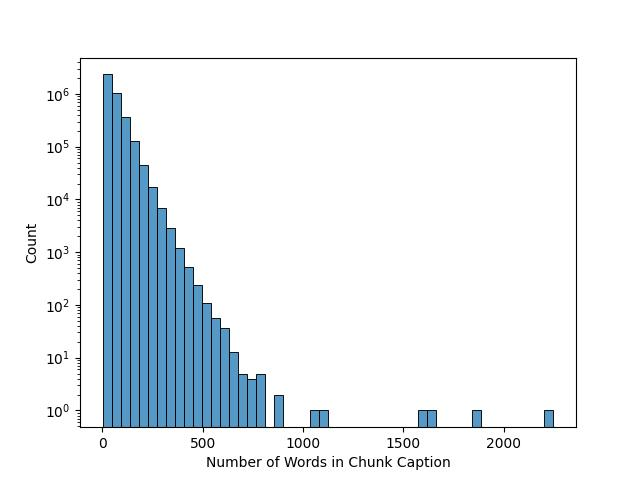
\includegraphics[width=\textwidth]{figs/data-statistic/caption_lens_all.jpg}
    \caption{Chunk Caption Distribution.}
    \label{fig:subfig1}
  \end{subfigure}
  \hfill
  \begin{subfigure}{0.45\textwidth}
    \centering
    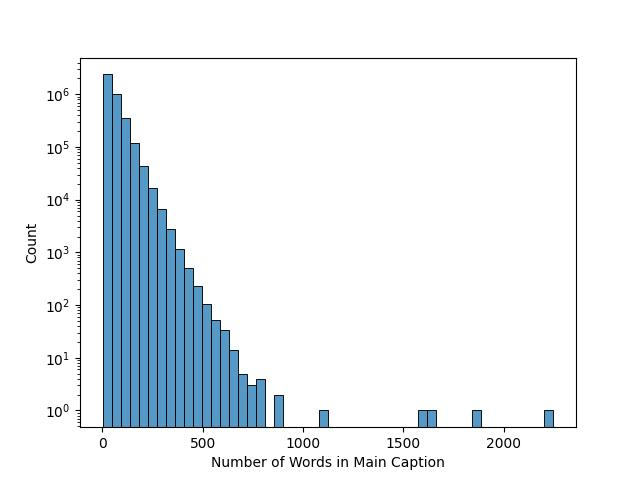
\includegraphics[width=\textwidth]{figs/data-statistic/caption_lens.jpg}
    \caption{Main Caption Distribution.}
    \label{fig:subfig2}
  \end{subfigure}
  \hfill
  \begin{subfigure}{0.45\textwidth}
    \centering
    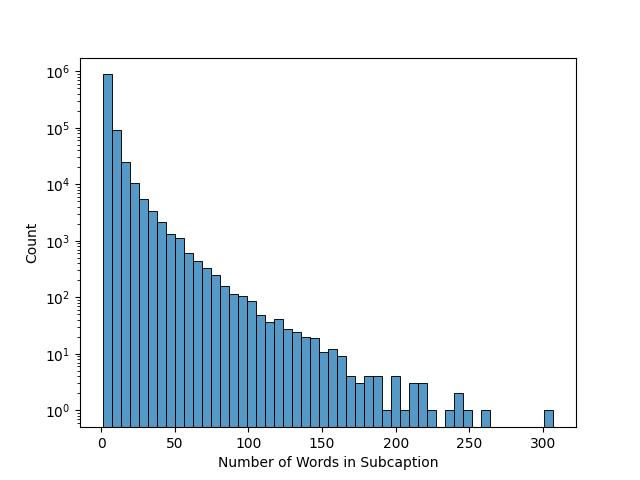
\includegraphics[width=\textwidth]{figs/data-statistic/sub_caption_lens.jpg}
    \caption{Subcaption Distribution.}
    \label{fig:subfig2}
  \end{subfigure}

  \caption{Caption Statistic.}
  \label{fig:caption-statistic}
\end{figure}